\documentclass[11pt,final,oneside]{fithesis}
\usepackage[utf8]{inputenc}
\usepackage[T1]{fontenc}
\usepackage{tipa}
\usepackage[slovak]{babel}
\usepackage{tabularx}
\usepackage{graphicx}
\usepackage{cite}
\usepackage{url}

\hbadness=1000
\tolerance=1000

\newcommand{\smalltt}[1]{\small\texttt{#1}\normalsize}

\thesistitle{Monitorování zátěže a využití výpočetních zdrojů v heterogenním výpočetním prostředí}
\thesissubtitle{Diplomová práca}
\thesisstudent{Juraj Leždík}
\thesiswoman{false}
\thesisfaculty{fi}
\thesisyear{jar 2016}
\thesisadvisor{Mgr. Miroslav Ruda}
\thesislang{sk}
\begin{document}

\FrontMatter
\ThesisTitlePage

\begin{ThesisDeclaration}
\DeclarationText
\AdvisorName
\end{ThesisDeclaration}


\begin{ThesisThanks}
\end{ThesisThanks}

\begin{ThesisAbstract}
\end{ThesisAbstract}

\begin{ThesisKeyWords}
\end{ThesisKeyWords}

\tableofcontents
\addcontentsline{toc}{chapter}{Obsah}

\MainMatter
\chapter{Úvod}

\chapter{Zber a uchovavanie časových rád}
\section{OpenTSDB}
OpenTSDB pozostáva z Time Series Daemon (TSD) a z utilít pre príkazový riadok. Interakcia s OpenTSDB je primárne realizovaná cez jedného alebo viacerých TSD. Každý TSD je nezávislý.
Neexistuje žiadny riadiaci proces, žiadny zdieľaný stav, takže je možné spustiť toľko TSD, koľko je potrebné na zvládnutie požadovanej záťaže. Každý TSD používa open-source databázu HBase
na ukladanie a vyberanie dát časových rád. HBase schéma je vysoko optimalizovaná na rýchlu agregáciu podobných časových rád, aby minimalizovala požiadavky na úložný priestor. 
Používatelia TSD nemusia kpristupovať do HBase priamo. S TSD je možné komunikovať cez jednoduchý protokol podobný Telnetu, cez HTTP API alebo cez jednoduché GUI. Všetka komunikácia
sa deje na tom istom porte (TSD odhadne protokol klienta pohľadom na prvých niekoľko bajtov, ktoré obdrží).\cite{openTSDB}




\chapter{Aktuálne monitorovacie riešenia}
\section{Open-source}
\subsection{Nagios}
\subsubsection{PluginAPI}
Scripts and executables must do two things (at a minimum) in order to function as Nagios plugins:

Exit with one of several possible return values
Return at least one line of text output to STDOUT
The inner workings of your plugin are unimportant to Nagios. Your plugin could check the status of a TCP port, run a database query, check disk free space, or do whatever else it needs to check something. The details will depend on what needs to be checked - that's up to you.

Return Code

Nagios determines the status of a host or service by evaluating the return code from plugins. The following tables shows a list of valid return codes, along with their corresponding service or host states.

Plugin Return Code	Service State	Host State
0	OK	UP
1	WARNING	UP or DOWN/UNREACHABLE*
2	CRITICAL	DOWN/UNREACHABLE
3	UNKNOWN	DOWN/UNREACHABLE
Note Note: If the use_aggressive_host_checking option is enabled, return codes of 1 will result in a host state of DOWN or UNREACHABLE. Otherwise return codes of 1 will result in a host state of UP. The process by which Nagios determines whether or not a host is DOWN or UNREACHABLE is discussed here.

Plugin Output Spec

At a minimum, plugins should return at least one of text output. Beginning with Nagios 3, plugins can optionally return multiple lines of output. Plugins may also return optional performance data that can be processed by external applications. The basic format for plugin output is shown below:

TEXT OUTPUT | OPTIONAL PERFDATA
LONG TEXT LINE 1
LONG TEXT LINE 2
...
LONG TEXT LINE N | PERFDATA LINE 2
PERFDATA LINE 3
...
PERFDATA LINE N

The performance data (shown in orange) is optional. If a plugin returns performance data in its output, it must separate the performance data from the other text output using a pipe (|) symbol. Additional lines of long text output (shown in blue) are also optional.
https://assets.nagios.com/downloads/nagioscore/docs/nagioscore/3/en/pluginapi.html

\subsubsection{Timeouty}

Format:	service_check_timeout=<seconds>
Example:	service_check_timeout=60
This is the maximum number of seconds that Nagios will allow service checks to run. If checks exceed this limit, they are killed and a CRITICAL state is returned. A timeout error will also be logged.

There is often widespread confusion as to what this option really does. It is meant to be used as a last ditch mechanism to kill off plugins which are misbehaving and not exiting in a timely manner. It should be set to something high (like 60 seconds or more), so that each service check normally finishes executing within this time limit. If a service check runs longer than this limit, Nagios will kill it off thinking it is a runaway processes.
https://assets.nagios.com/downloads/nagioscore/docs/nagioscore/3/en/configmain.html#service_check_timeout



Nie je mechanizmus pre reštart alebo individuálne timeouty.
Má zastaralý Hadoop plugin, používa staré REST API.
Last Release Date 2010-11-05
https://exchange.nagios.org/directory/Plugins/Others/check_hadoop_metrics/details

\subsection{Zabbix}
\subsubsection{Timeouty}
Timeout processing
Zabbix will not process a simple check longer than Timeout seconds defined in Zabbix server configuration file.
https://www.zabbix.com/documentation/1.8/manual/config/items

Zabbix Agent
Timeout	 no	 1-30	3	Spend no more than Timeout seconds on processing
https://www.zabbix.com/documentation/1.8/manual/processes/zabbix_agentd

Zabbix Server
Timeout	 no	 1-30	3	Specifies how long we wait for agent, SNMP device or external check (in seconds).
https://www.zabbix.com/documentation/1.8/manual/processes/zabbix_server

NEuvádza sa nič o killovaní procesov.
\subsubsection{Moduly}

Loadable modules offer a performance-minded option for extending Zabbix functionality.

There already are ways of extending Zabbix functionality by way of:

user parameters (agent metrics)
external checks (agent-less monitoring)
system.run[] Zabbix agent item.
They work very well, but have one major drawback, namely fork(). Zabbix has to fork a new process every time it handles a user metric, which is not good for performance. It is not a big deal normally, however it could be a serious issue when monitoring embedded systems, having a large number of monitored parameters or heavy scripts with complex logic or long startup time.

Zabbix 2.2 comes with support of loadable modules for extending Zabbix agent, server and proxy without sacrificing performance.

A loadable module is basically a shared library used by Zabbix daemon and loaded on startup. The library should contain certain functions, so that a Zabbix process may detect that the file is indeed a module it can load and work with.

Loadable modules have a number of benefits. Great performance and ability to implement any logic are very important, but perhaps the most important advantage is the ability to develop, use and share Zabbix modules. It contributes to trouble-free maintenance and helps to deliver new functionality easier and independently of the Zabbix core code base.
https://www.zabbix.com/documentation/2.2/manual/config/items/loadablemodules


\subsection{Icinga}
By default the Icinga 2 daemon is running as icinga user and group using the init script. Using Debian packages the user and group are set to nagios for historical reasons.
http://docs.icinga.org/icinga2/latest/doc/module/icinga2/toc#!/icinga2/latest/doc/module/icinga2/chapter/getting-started#running-icinga2

\subsubsection{Externé pluginy}
Icinga determines the status of a host or service by evaluating the return code from plugins. The following tables shows a list of valid return codes, along with their corresponding service or host states
http://docs.icinga.org/latest/en/pluginapi.html

\subsubsection{Notifikácie a príkazy udalostí}
Unlike notifications, event commands for hosts/services are called on every check execution if one of these conditions match:
The host/service is in a soft state
The host/service state changes into a hard state
The host/service state recovers from a soft or hard state to OK/Up

Ide len o spustenie nejakého systémového príkazu.
http://docs.icinga.org/icinga2/latest/doc/module/icinga2/toc#!/icinga2/latest/doc/module/icinga2/chapter/monitoring-basics#event-commands

\subsubsection{Itegrácie s aplikáciami} 
Docker
https://www.icinga.org/products/integrations/
these tiny pure shell+awk plugins for monitoring your hadoop cluster are a enhanced and uptodate version of exchange.nagios.org check_hadoop-dfs.sh
https://github.com/noqqe/icinga-hadoop-plugins

\subsection{Cacti} 
Cacti is a complete network graphing solution designed to harness the power of RRDTool's data storage and graphing functionality. Cacti provides a fast poller, advanced graph templating, multiple data acquisition methods, and user management features out of the box.
http://www.cacti.net/

\subsection{collectd}
There are some key differences we think set collectd apart. For one, it's written in C for performance and portability, allowing it to run on systems without scripting language or cron daemon, such as embedded systems. 
At the same time it includes optimizations and features to handle hundreds of thousands of data sets. It comes with over 90 plugins. It provides powerful networking features and is extensible in numerous ways. 

\subsubsection{Obmedzenia}
It does not generate graphs. It can write to RRD files, but it cannot generate graphs from these files. 
Monitoring functionality has been added in version 4.3, but is so far limited to simple threshold checking. 
https://collectd.org/index.shtml

\subsubsection{Zapisovací plugin Write TSDB}
The Write TSDB plugin writes metrics to OpenTSDB, an open-source distributed time-series database based on Apache HBase.
https://collectd.org/wiki/index.php/Plugin:Write_TSDB

\begin{description}
\item[\emph{Host Address}] Hostname or address to connect to. Defaults to localhost.
\item[\emph{Port Service}] Service name or port number to connect to. Defaults to 4242.
\item[\emph{HostTags String}] When set, HostTags is added to the end of the metric. It is intended to be used for name=value pairs that the TSD will tag the metric with. Dots and whitespace are not escaped in this string.
\item[\emph{StoreRates false|true}] If set to true, convert counter values to rates. If set to false (the default) counter values are stored as is, as an increasing integer number.
\item[\emph{AlwaysAppendDS false|true}] If set the true, append the name of the Data Source (DS) to the "metric" identifier. If set to false (the default), this is only done when there is more than one DS.
\end{description}

\subsubsection{Prahy a notifikácie}

The only action the Threshold plugin takes itself is to generate and dispatch a notification. Every time a value is out of range, 
notification is dispatched. 
Also, all values that match a threshold are considered to be relevant or "interesting". As a consequence collectd will issue a notification 
if they are not received for Timeout iterations.  for example, Timeout is set to "2" (the default) and some hosts sends it's CPU statistics to the server every 60 seconds, a notification will be dispatched after about 120 seconds. It may take a little longer because the timeout is checked only once each Interval on the server.

When a value comes within range again or is received after it was missing, an "OKAY-notification" is dispatched.
https://collectd.org/documentation/manpages/collectd-threshold.5.shtml

https://collectd.org/wiki/index.php/Plugin:Write_TSDB

\subsection{Problém s reakciami na prahové hodnoty}
Všetky tieto aplikácie poskytujú mechanizmus na reagovanie na nezvyčajné udalosti. Ak je meraná hodnota mimo určitý rozsah, je generované hlásenie. Na to je možné reagovať.
Na situáciu, keď časť zodpovedná za zberanie dát nejakej metriky neodpovedá, je ale možné reagovať len reštartovaním celej monitorovacej aplikácie. 
Nie je možné jednotlivé moduly ovládať nezávisle. 
Preto bude potrebné vytvoriť niektoré moduly tak, aby jedna časť bola neustále dostupná a reagovala na výzvy od riadiacej aplikácie.

\subsection{Ostatne} 
\begin{description}
\item[\emph{Zenoss}]
\item[\emph{Munin}]
\end{description}

\section{Ganglia} 
Ganglia is a scalable distributed monitoring system for high-performance computing systems such as clusters and Grids. It is based on a hierarchical design targeted at federations of clusters. It leverages widely used technologies such as XML for data representation, XDR for compact, portable data transport, and RRDtool for data storage and visualization. It uses carefully engineered data structures and algorithms to achieve very low per-node overheads and high concurrency. The implementation is robust, has been ported to an extensive set of operating systems and processor architectures, and is currently in use on thousands of clusters around the world. It has been used to link clusters across university campuses and around the world and can scale to handle clusters with 2000 nodes.
Ganglia is a BSD-licensed open-source project that grew out of the University of California, Berkeley Millennium Project
ttp://ganglia.info/
Monitoring plugin pre hadoop
http://ganglia.info/?p=88
O tom ako funguju notifikacie som nic nenasiel.

\section{Komerčné riešenia}


\section{Torque}
Nenašiel som žiadne komerčný software na monitorovanie tohto softvéru. 

\section{libvirt/KVM}

\section{Docker}
\subsection{Scout}
Scout runs within Docker containers without any special configuration. \cite{scout}

\subsection{New Relic}
http://newrelic.com/docker

\subsection{AppDynamics}
https://www.appdynamics.com/community/exchange/extension/docker-monitoring-extension/


\section{Hadoop}
\subsection{New Relic}
http://newrelic.com/plugins
\subsection{AppDynamics}
The Hadoop monitoring extension captures metrics from Hadoop Resource Manager and/or Apache Ambari and displays them in Appdynamics Metric Browser.

This extension works only with the standalone machine agent.


Metrics include:

Hadoop Resource Manager
App status and progress: submitted, pending, running, completed, killed, and failed app count
Memory size, memory usage
Allocated containers, container count in different states
Node status, count of nodes in different states
Scheduler capacity, app and container count
Ambari
Individual host metrics including CPU, disk, memory, JVM, load, network, process, and RPC metrics
Service component metrics including CPU, disk, memory, JVM, load, network, process, RPC, and component-specific metrics

https://www.appdynamics.com/community/exchange/extension/hadoop-monitoring-extension/

\chapter{Oblasti monitorovania}
\section{Torque}
TORQUE Resource Manager poskytuje kontrolu nad dávkovými úlohami a distribuovanými výpočetnými zdrojmi. Je to pokročilý open-source product, založený na na pôvodnom PBS projekte. 
Zahŕňa vyznamné pokroky v oblastiach škálovania, spoľahlivosti a funkcionality a je v súčasnosti používaný desiatkami tisícov vládnych, akademických a komerčných webových stránok po celom svete. Torque môže byť voľne používaný, modifikovaný a distribuovaný je v rámci obmedzení svojou licenciou.\cite{torque}

Monitorovanie tejto aplikácie bude prebiehat prostredníctvom volania jej ovládacích príkazov:
\begin{description}
\item[\emph{momctl}] - sledovanie záťaže riadiaceho procesu a zisťovanie, ktoré úlohy sa práve spracovávajú
\item[\emph{printjob}] - sledovanie zdrojov, ktoré spotrebováva konkrétna úloha 
\end{description}



\section{Docker}
Docker umožňuje zabaliť aplikáciu so všetkými jej závislosťami do štandardizovanej jednotky určenej na softvérový vývoj. Kontajnery Dockeru obaľujú softvér kompletným súborovým systémom, ktorý
zahŕňa všetko, čo daný softvér potrebuje na spustenie: kód, nástroje potrebné na beh, systémové nástroje a knižnice. Toto zaručuje, že program bude pracovať rovnako bez ohľadu na prostredie, v ktorom
je spustený.\cite{docker}




\subsection{Porovnanie s virtuálnymi strojmi}
Kontajnery predstavujú podobný prístup ako virtualizácia. Tiež ide o snahu spúšťať softvér v prostredí oddelenom od skutočného hardvéru a operačného systému. Na rozdiel od úplných virtuálnych strojov 
nie je virtualizovaný celý hardvér, ale len softvérové vybavenie nevyhnutné na spustenie programu. Rozdiel v architektúre ilustruje nasledovný obrázok: 
\begin{figure}[h]
\begin{center}
       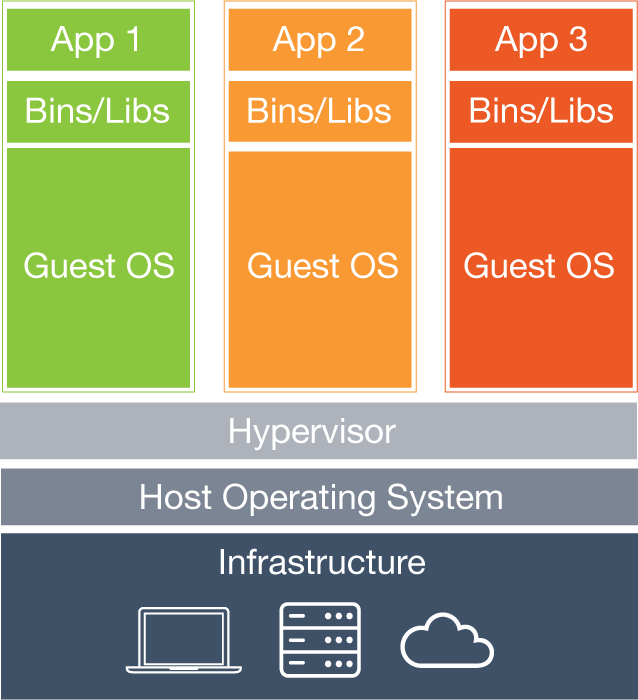
\includegraphics[width=0.8\textwidth]{images/docker.png}
       \caption{Porovnanie architektúry Docker a virtuálnych strojov}\cite{docker}
\end{center}
\end{figure}

\subsection{Komunikácia s Dockerom}
Na komunikáciu s Dockerom je možné využiť:
\begin{description}
\item[príkazy aplikácie v príkazovom riadku]
\item[Remote API]
\end{description}

Používanie príkazov aplikácie môže byť o čosi rýchlejšie, ale následne by bolo potrebné analyzovať textový výstup programu.
Rozhodol som sa použiť Remote API. Toto API funguje pre účely monitorovania na princípe REST a odpovede vracia vo formáte JSON, čo predstavuje zjednodušenie spracovania výstupu. Démon Dockeru "počúva" na 
lokálnom sockete, čo by nemalo spôsobovať výrazné oneskorenie odpovede.

O každom kontajneri spustenom v Dockeri budem sledovať využívanie týchto zdrojov :
\begin{description}
\item[\emph{procesor}]
\item[\emph{pevný disk}]
\item[\emph{sieť}]
\item[\emph{pamäť}]
\end{description}

  
Dáta je možné zberať buď ako prúd, alebo po jednorazových žiadostiach. To ešte nemám veľmi preštudované, neviem aké sú tam intervaly, tak sa rozhodnem až neskôr.
Predpokladám ale, že z hľadiska rýchlosti a alokácie bude cesta asi ten stream.

\section{libvirt/KVM}
KVM\footnotemark\footnotetext{Kernel-based Virtual Machine} je plné virtualizačné riešenie pre Linux pre x86 hardvér, obsahujúce virtualizačné rozšírenia (Intel VT or AMD-V).
Pozostáva z nahrateľného modulu jadra, kvm.ko, ktorý poskytuje základ virtualizačnej infraštruktúry a šepcifický modul, kvm-intel.ko alebo kvm-amd.ko. Je možné virtualizovať obrazy 
s operačným systémami Linux aj Windows. Každý virtuálny stroj má vlastný virtualizovaný hardvér: sieťovú kartu, disk, grafický adaptér, atď. KVM je open-source softvér. Virtualizačný modul jadra
sa nachádza v Linuxe od verzie 2.6.20.\cite{torque}

libvirt je sada nástrojov na prácu s virtualizačnými schopnosťami Linuxu (a ostatných OS). Je to voľný softvér dostupný pod licenciou GNU LGPL. 
Obsahuje API v jazyku C a väzby pre bežné programovacie jazyky.\cite{libvirt}

Na monitorovanie virtuálnych strojov použijem API libvirt v jazyku Python. Budem sledovať využívanie nasledujúcich zdrojov vo virtuálnom stroji:
\begin{description}
\item[\emph{procesor}]
\item[\emph{pevný disk}]
\item[\emph{sieť}]
\end{description}

libvirt momentálne neposkytuje nástroje na monitorovanie spotreby pamäte.


Využijem už existujúcu implementáciu sond na zber týchto údajov (aspoň teda myslím).


\section{Hadoop}
Projekt Apache™ Hadoop® vyvíja open-source softvér na spoľahlivé, škálovateľné, distribuované výpočty. Apache Hadoop je prostredie, ktoré umožňuje distribuované spracovávanie veľkých množstiev dát
naprieč clustermi, používajúcimi jednoduché programovacie modely. Je navrhnutý tak, aby bol škálovateľný od jednotlivých serverov po tisícky strojov, kde každý poskytuje lokálny výpočetný výkon a úložný priestor.
Nespolieha sa na vysokú dosupnosť hardvérových prostriedkov, ale je navrhnutý, aby detekoval a zvládal chyby na aplikačnej vrstve, takže poskytuje vysoko dostupnú službu nad clusterom počítačov, z ktorých 
každý je náchylný na chyby.

Projekt pozostáva z týchto modulov:

\begin{description}
\item[\emph{Hadoop Common:}] spoločné nástroje, ktoré podporujú ostatné Hadoop moduly
\item[\emph{Hadoop Distributed File System (HDFS™):}] distribuovaný súborový systém, ktorý poskytuje vysokú priepustnosť
\item[\emph{Hadoop YARN:}] prostredie pre plánovanie úloh a správu zdrojov clustera
\item[\emph{Hadoop MapReduce:}] systém založený na YARN pre paralelné spracovávanie veľkých množstiev dátprostredie pre plánovanie úloh a správu zdrojov clustera
\end{description}

\section{Monitoring cez Hadoop YARN REST API}
The Hadoop YARN web service REST APIs are a set of URI resources that give access to the cluster, nodes, applications, and application historical information. The URI resources are grouped into APIs based on the type of information returned. Some URI resources return collections while others return singletons.
HTTP Requests

To invoke a REST API, your application calls an HTTP operation on the URI associated with a resource.

Summary of HTTP operations

Currently only GET is supported. It retrieves information about the resource specified.

Security

The web service REST API’s go through the same security as the web UI. If your cluster adminstrators have filters enabled you must authenticate via the mechanism they specified.

https://hadoop.apache.org/docs/current/hadoop-yarn/hadoop-yarn-site/WebServicesIntro.html

A že štatistiky sa ukaladajú aj niekam na HDFS, ale zrejme v nejakom XML internéhomakd
formátu. Takisto by som potreboval skonzultovať, že čo vlastne monitorovať.

\chapter{Metriky}
\section{Torque}
\subsection{Technika zbierania metrík}
Na zbieranie metrík som použil príkaz \emph{qstat -j}.

			Prints either for all pending jobs  or  the  jobs  con-
          tained  in  job_list  various information. The job_list
          can contain job_ids, job_names, or wildcard  expression
          sge_types(1).

          For  jobs  in  E(rror)  state  the  error   reason   is
          displayed. For jobs that could not be dispatched during
          in the  last  scheduling  interval  the  obstacles  are
          shown, if 'schedd_job_info' in sched_conf(5) is config-
          ured accordingly.

          For running  jobs  available  information  on  resource
          utilization   is  shown  about  consumed  cpu  time  in
          seconds,  integral  memory  usage  in  Gbytes  seconds,
          amount  of  data  transferred in io operations, current
          virtual memory utilization in Mbytes, and maximum  vir-
          tual  memory utilization in Mbytes. This information is
          not available if resource utilization retrieval is  not
          supported for the OS platform where the job is hosted.
\subsection{Zbierané metriky}
Príkaz qstat -j poskytuje viacero režimov výstupu.
\begin{description}
\item[\emph{Cluster Queue Format}]
		\\the cluster queue name.

     \\ an average of the normalized load average  of  all  queue
        hosts.  

    \\  the number of currently used slots.

     \\  the number of slots reserved in advance.

     \\  the number of currently available slots.

    \\  the total number of slots.

     \\  the number of slots which is  in  at  least  one  of  the
        states  'aoACDS' and in none of the states 'cdsuE'

     \\ the number of slots which are in one of these  states  or
        in any  combination of them: 'cdsuE'

\item[\emph{Reduced Format}]
	\\the job ID.

     \\ the priority of the job determining its position  in  the
        pending  jobs  list. 

    \\  the name of the job.

     \\  the user name of the job owner.

     \\ the status of the  job  -  one  of  d(eletion),  E(rror),
        h(old), r(unning), R(estarted), s(uspended), S(uspended),
        t(ransfering), T(hreshold) or w(aiting).

     \\  the submission or start time and date of the job.

     \\  the  queue  the  job  is  assigned  to  (for  running  or
        suspended jobs only).

     \\  the number of job slots or the function of  parallel  job
        tasks if -g t is specified.

     \\  the array job task id. Will be empty for non-array  jobs.
        See  the  -t option to qsub(1) and the -g above for addi-
        tional information.

     If the -t option is supplied, each status line  always  con-
     tains  parallel  job task information as if -g t were speci-
     fied and each line contains the following parallel job  sub-
     task information:
     \\  the parallel task ID (do not confuse parallel tasks  with
        array job tasks),

     \\  the status of the  parallel  task  -  one  of  r(unning),
        R(estarted),   s(uspended),   S(uspended),   T(hreshold),
        w(aiting), h(old), or x(exited).

     \\  the cpu, memory, and I/O usage,

     \\ the exit status of the parallel task,

     \\  and the failure code and message for the parallel task.
\item[\emph{Full Format}]
the queue name,

     \\  the  queue  type  -  one   of   B(atch),   I(nteractive),
        C(heckpointing),  P(arallel),  T(ransfer) or combinations
        thereof or N(one),

     \\  the number of used and available job slots,

     \\  the load average of the queue host,

     \\  the architecture of the queue host and

     \\  the state  of  the  queue  -  one  of  u(nknown)  if  the
        corresponding  sge_execd(8) cannot be contacted, a(larm),
        A(larm),     C(alendar      suspended),      s(uspended),
        S(ubordinate),  d(isabled), D(isabled), E(rror) or combi-
        nations thereof.

     \\resource availability information
     is  printed  following  the  queue  status  line.  

     \\  the job ID,

     \\  the priority of the job determining its position  in  the
        pending  jobs  list.  

     \\  the job name,

     \\  the job owner name,

     \\  the status of the job - one of t(ransfering),  r(unning),
        R(estarted), s(uspended), S(uspended) or T(hreshold) (see
        the Reduced Format section for detailed information),

     \\  the submission or start time and date of the job.

     \\  the number of job slots or the function of  parallel  job
        tasks if -g t is specified.


     \\If the -t option is supplied, each job status line also con-
     tains

     \\  the task ID,

     \\  the status of the task - one of  r(unning),  R(estarted),
        s(uspended), S(uspended), T(hreshold), w(aiting), h(old),
        or x(exited) (see the Reduced Format section for detailed
        information),

     \\  the cpu, memory, and I/O usage,

     \\  the exit status of the task,

     \\  and the failure code and message for the task.

\end{description}
 
Potrebné metriky poskytuje prepínač -t v redukovanom formáte, preto som použil túto metódu výstupu.

\section{Docker}
O každom kontajneri je možné zberať metriky o tom, ako spotrebováva zdroje.
\subsection{Sieť}
Aby mohli medzi sebou jednotlivé kontajnery komunikovať, Docker im poskytuje sieťové rozhrania. Každé rozhranie má nakonfigurovanú sieť,
do ktorje patrí. Na to, aby kontajnery spolu mohli komunikovať, musia byť členmi rovnakej siete. Komunikácia naprieč sieťami nie je možná.
Užívatelia si môžu definovať vlastné siete. Docker na vytvorenie týchto sietí poskytuje dva ovládače.

\subsubsection{Sieť typu most}
Je to jednoduchý typ siete určený pre malé siete. Je ju možné vytvoriť príkazom 
\\
{\em \$ docker network create --driver bridge NÁZOV_SIETE }
\\
Po vytvorení siete je možné spustiť kontajnery v tejto sieti príkazom
\\
{\em \$ docker run --net=NÁZOV_SIETE --name= NÁZOV_KONTAJNERA}
\\

\subsubsection{Prekladaná sieť}
Docker umožňuje vytvoriť aj sieť, v ktorej sa nachádza viacero hostov zároveň. To umožňuje komunikovať medzi sebou aj kontajnerom,
ktoré sú spustené v rozličných k a ani na jednom hoste.
An overlay network

\subsubsection{Metriky siete}
Pre jednotlivé sieťové rozhrania je možné zbierať tieto metriky:

\\    rx_bytes
\\    rx_dropped
\\    rx_error
\\    rx_packets
\\    tx_bytes
\\    tx_dropped
\\    tx_errors
\\    tx_packets

\subsection{Pamäť}
\\        usage - spotreba pamäte
\\        failcnt - počet chýb

\subsection{Procesor}
\\        cpu_usage 
\\           percpu_usage
\\              16970827,
\\              1839451,
\\              7107380,
\\              10571290
\\           usage_in_usermode"
\\           total_usage" 
\\           usage_in_kernelmode" 
\\        system_cpu_usage

\section{libvirt/KVM}

\section{Hadoop}

\chapter{Návrh}
Monitorovacia aplikácia bude pozostávať z dvoch častí. Jednou bude manažér a druhou monitorovacie sondy. Manažér bude oslovovať jednotlivé sondy v pravidelných intervaloch, aby mu poslali údaje o zaťažení.
Tieto údaje následne bude odosielať TSD. Manažér bude napísaný v Go a bude využívať Go rutiny (niečo ako vlákna) - jednu pre každú sondu.

V prípade napr. toho Torque sme sa bavili, že je možné, že na dotaz o zaťažení môže trvať v niektorých prípadoch aj polhodinu, kým príde odpoveď. V princípe nejde nijako odlíšiť, či daná sonda čaká na údaje
alebo sa zasekla. Preto každá sonda bude obsahovať časť, ktorá bude stále živá a bude komunikovať s manažérom. Buď mu pošle nové údaje, alebo povie, že čaká. V tom prípade manažér použije poslednú hodnotu.
V prípade, že sonda bude čakať na údaj, nebudú sa vytvárať nové požiadavky na tento údaj. Opätovný dotaz na údaje bude vytvorený až po uplynutí nejakého časového intervalu a starý dotaz bude zrušený/ukončený.
Tento časový interval si bude môcť užívateľ nastaviť pre každú sondu. Zároveň by som chcel ale otestovať v reálnom prostredí, aký interval by bol vhodný pre tú ktorú sondu.

Ďalšou vecou na riešenie by bolo zabezpečenie dát. To ale momentálne nie je podporované v OpenTSDB, tak by šlo len o teoretické rozobratie. Ďalšie nové veci, už teraz nevymyslím, najprv treba niečo nakódiť
a objaviť komplikácie.

\chapter{Záver}

\bibliographystyle{csplainurl}
\nocite{*}
\bibliography{dip-lezdik}
\addcontentsline{toc}{chapter}{Literatúra}

\begin{appendix}
\chapter{Kapitola priloha}
\end{appendix}

\end{document}
